\documentclass[aspectratio=169, 10pt]{beamer}
\usetheme{Boadilla}
\usecolortheme{seahorse}

\usepackage{graphicx}
\usepackage{caption}
\usepackage{subcaption}

\setbeamertemplate{caption}[numbered]
\setbeamerfont{caption}{size=\scriptsize}

\title[S\&P 500 Financial Network]{Structural and Influence Analysis of Financial Systems}
\subtitle{S\&P 500 Correlation Network}
\author{Network Science Project}
\date{\today}

\begin{document}

\begin{frame}
    \titlepage
\end{frame}

\begin{frame}{Outline}
    \tableofcontents
\end{frame}

% ---------------------------------------------------------
\section{Network Construction}
% ---------------------------------------------------------
\begin{frame}{Network Construction}
    \begin{columns}[c]
        \begin{column}{0.5\textwidth}
            \textbf{Problem:} 
            \vspace{0.1cm}
            \\
            Raw Pearson correlations are dominated by the common market factor, producing a dense, uninformative graph.
            
            \vspace{0.3cm}
            \textbf{Methodology:}
            \begin{itemize}
                \item 2-year daily log-returns for $N=501$ stocks.
                \item \textbf{Market-mode filtering} (Onnela et al.\ 2003): subtracted equal-weight market index.
                \item \textbf{Thresholding}: edges where $|\rho| > 0.3$.
            \end{itemize}
            
            \vspace{0.3cm}
            \textbf{Result:} Mean $|\rho|$ fell from $0.235 \to 0.127$; the filtered graph has $10{,}002$ edges.
        \end{column}
        
        \begin{column}{0.45\textwidth}
            \begin{figure}
                \centering
                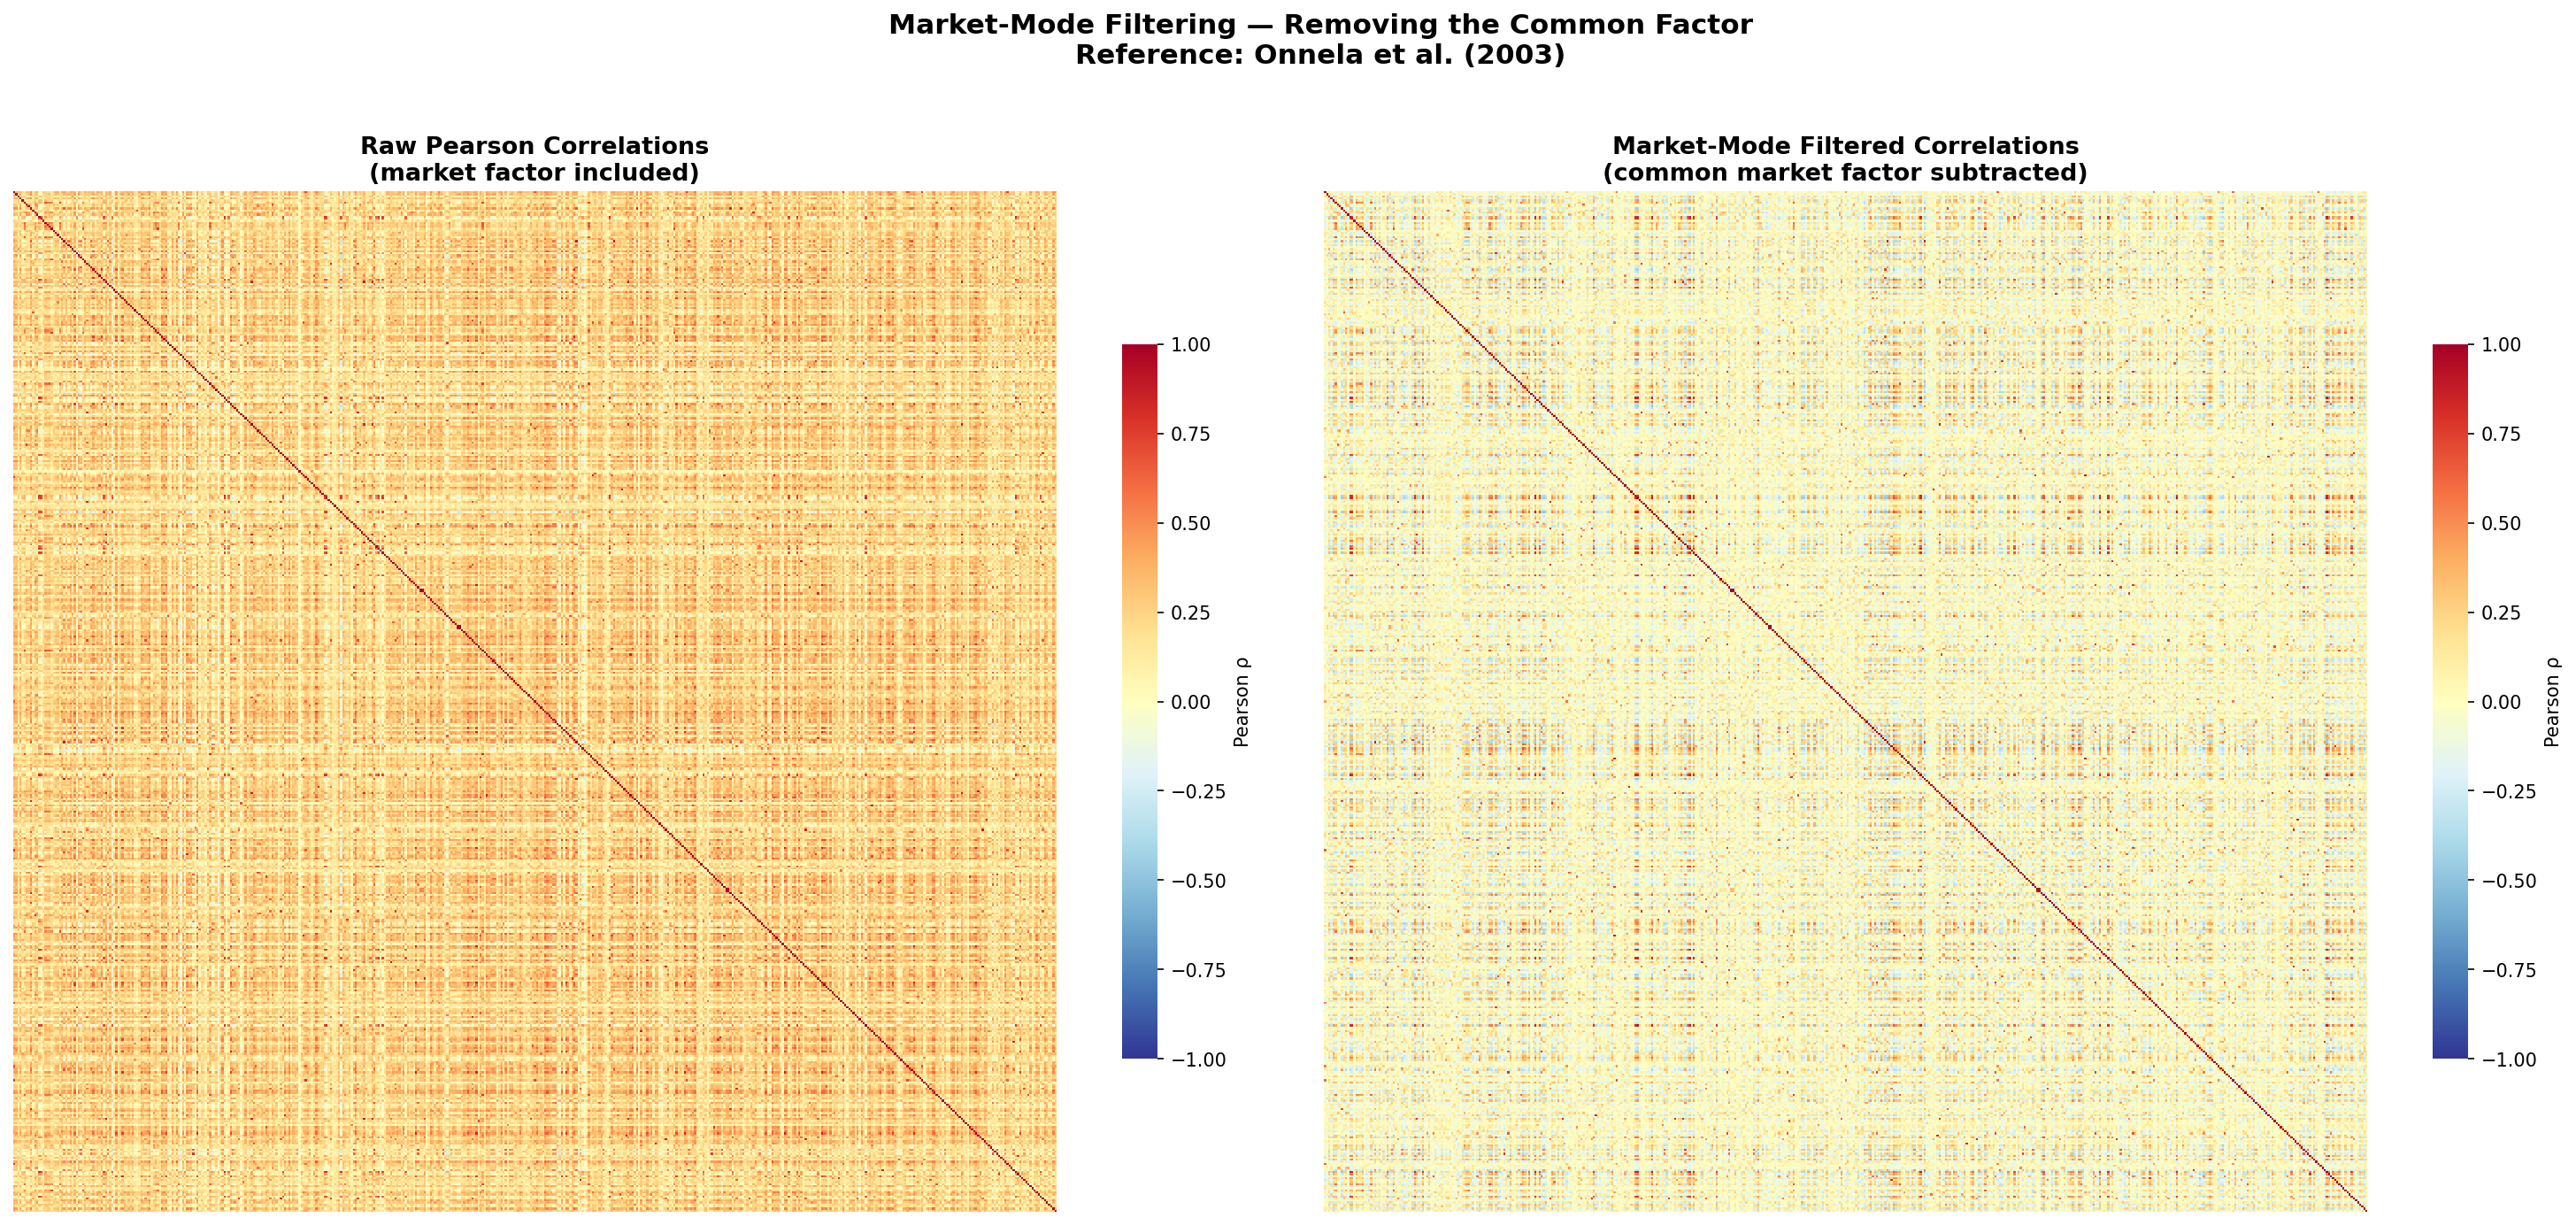
\includegraphics[width=\linewidth,height=0.7\textheight,keepaspectratio]{../../figures/correlation_heatmap_comparison.png}
                \caption{Raw vs.\ filtered correlation heatmap.}
            \end{figure}
        \end{column}
    \end{columns}
\end{frame}

% ---------------------------------------------------------
\section{Scale-Free Analysis}
% ---------------------------------------------------------
\begin{frame}{Degree Distribution}
    \begin{columns}[c]
        \begin{column}{0.5\textwidth}
            \textbf{Connectivity}
            \begin{itemize}
                \item 47 connected components; Giant Component holds $89.4\%$ of all nodes.
            \end{itemize}

            \vspace{0.2cm}
            \textbf{Power-Law Fit} (Clauset et al.\ 2009)
            \begin{itemize}
                \item Heavy-tailed degree distribution.
                \item $P(k) \sim k^{-\gamma}$, \; $\gamma \approx 2.14$.
                \item Confirms hub-dominated, scale-free topology.
            \end{itemize}
        \end{column}
        
        \begin{column}{0.45\textwidth}
            \begin{figure}
                \centering
                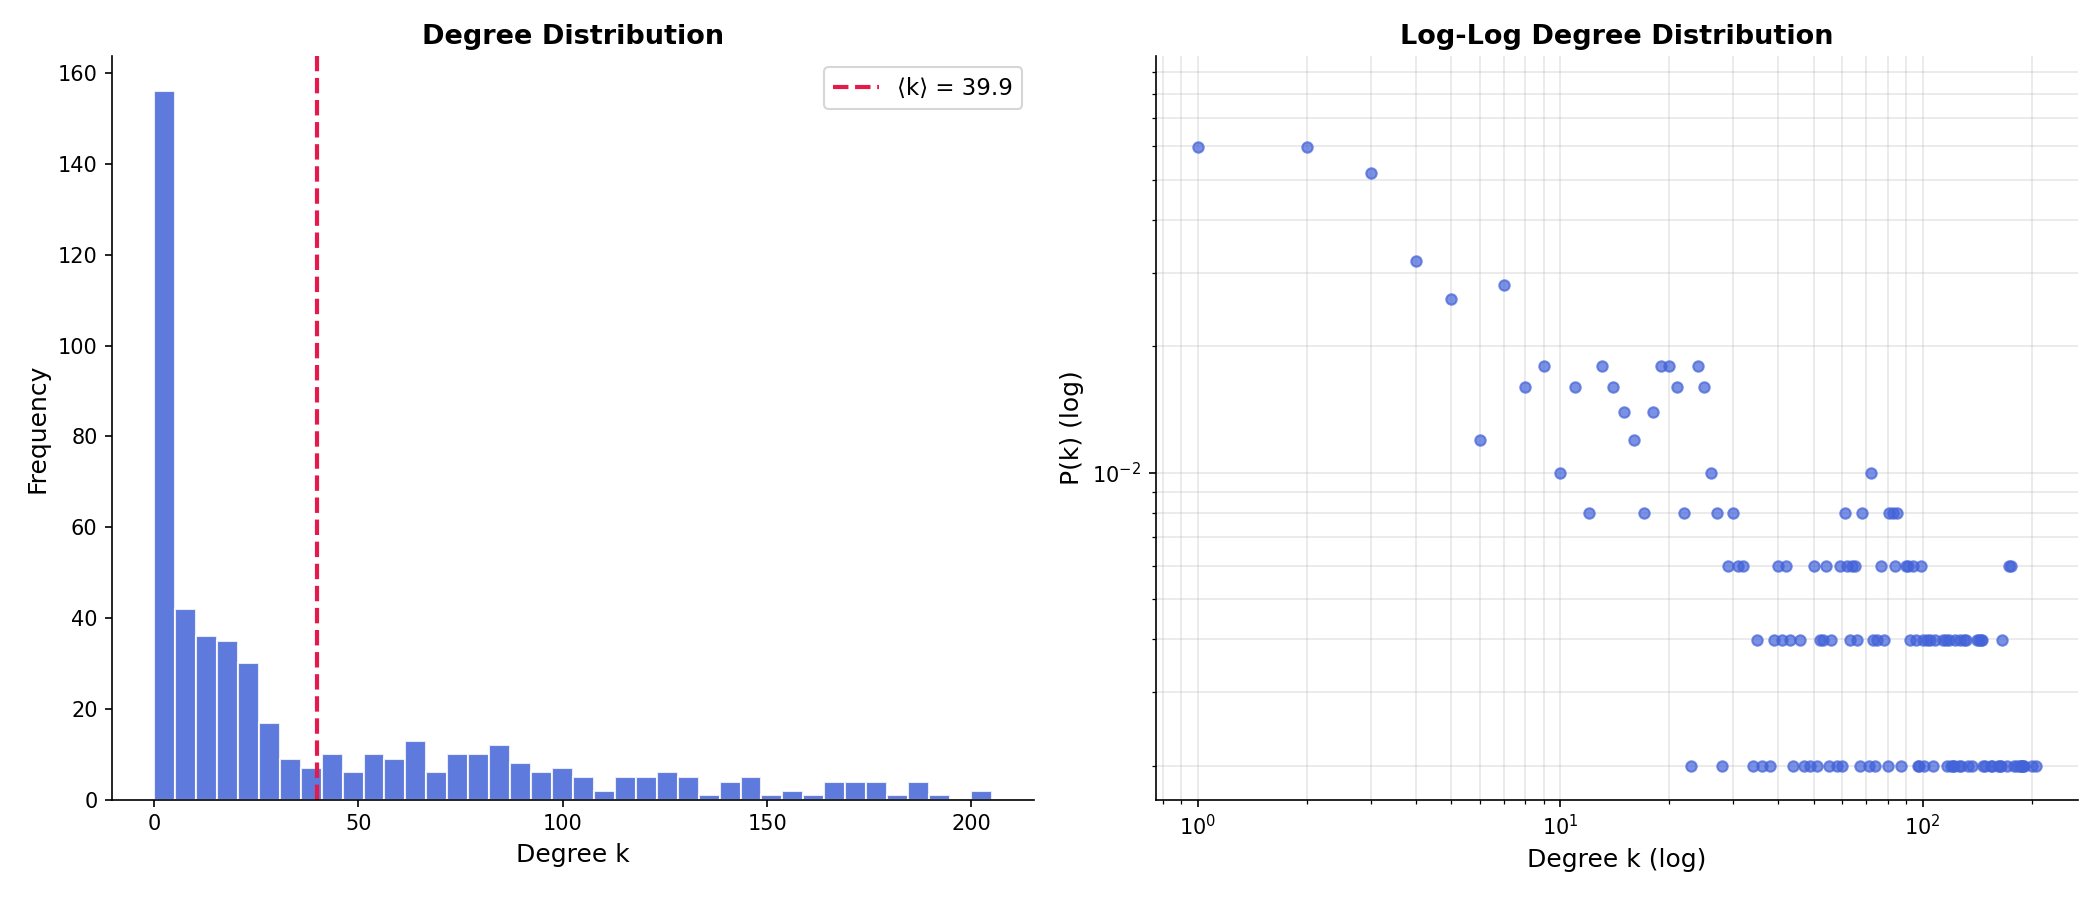
\includegraphics[width=\linewidth,height=0.45\textheight,keepaspectratio]{../../figures/degree_distribution.png}
                \vspace{0.1cm}
                
\includegraphics[width=\linewidth,height=0.45\textheight,keepaspectratio]{../../figures/powerlaw_fit.png}
            \end{figure}
        \end{column}
    \end{columns}
\end{frame}

\begin{frame}{Small-World}
    \begin{columns}[c]
        \begin{column}{0.5\textwidth}
            \textbf{ER Baseline}
            \begin{itemize}
                \item Against Erd\H{o}s--R\'enyi: $\sigma_{ER} = 4.56$.
                \item ER underestimates clustering due to ignoring degree heterogeneity.
            \end{itemize}
            
            \vspace{0.2cm}
            \textbf{Configuration Model}
            \begin{itemize}
                \item Degree-preserving null model gives $\sigma_{config} = 1.75$; still $> 1$.
                \item Bootstrap ($B=200$): $p < 0.001$, confirming significance.
                \item Weighted clustering $C^{w} = 0.22$ vs.\ unweighted $C = 0.64$ (Barrat et al.\ 2004).
            \end{itemize}
        \end{column}

        \begin{column}{0.45\textwidth}
            \begin{figure}
                \centering
                
\includegraphics[width=\linewidth,height=0.45\textheight,keepaspectratio]{../../figures/er_comparison.png}
                \vspace{0.1cm}
                
\includegraphics[width=\linewidth,height=0.45\textheight,keepaspectratio]{../../figures/bootstrap_distributions.png}
            \end{figure}
        \end{column}
    \end{columns}
\end{frame}

% ---------------------------------------------------------
\section{Contagion}
% ---------------------------------------------------------
\begin{frame}{Influence Propagation}
    \begin{columns}[c]
        \begin{column}{0.5\textwidth}
            \textbf{Cascade Model}
            \begin{itemize}
                \item Degree centrality vs.\ cascade spread: $r = -0.61$. High-degree nodes dilute per-edge impact through row-normalised weights.
            \end{itemize}
            \vspace{0.3cm}
            \textbf{Robustness} (Barab\'asi Ch.\ 8)
            \begin{itemize}
                \item Random failure: GCC degrades gracefully (scale-free resilience).
                \item Targeted betweenness attack: GCC collapses rapidly.
            \end{itemize}
        \end{column}
        
        \begin{column}{0.45\textwidth}
            \begin{figure}
                \centering
                
\includegraphics[width=\linewidth,height=0.65\textheight,keepaspectratio]{../../figures/robustness_analysis.png}
                \caption{Robustness under random vs.\ targeted attack.}
            \end{figure}
        \end{column}
    \end{columns}
\end{frame}

% ---------------------------------------------------------
\section{Event Validation}
% ---------------------------------------------------------
\begin{frame}{Event Validation}
    \begin{columns}[c]
        \begin{column}{0.5\textwidth}
            \textbf{Approach}
            \vspace{0.2cm}
            \\
            Rather than synthetic shocks, we seed propagation with actual event-day returns and compare model predictions against realised post-event performance.
            
            \vspace{0.3cm}
            \textbf{Scenarios:}
            \begin{itemize}
                \item AI / Semiconductor Rally (Jul 2024)
                \item Yen Carry-Trade Unwind (Aug 2024)
                \item Tariff Shock (Apr 2025)
            \end{itemize}
        \end{column}
        
        \begin{column}{0.45\textwidth}
            \begin{figure}
                \centering
                
\includegraphics[width=\linewidth,height=0.65\textheight,keepaspectratio]{../../figures/AI_Semiconductor_Rally_validation.png}
                \caption{Model vs.\ actual 5-day returns.}
            \end{figure}
        \end{column}
    \end{columns}
\end{frame}

% ---------------------------------------------------------
\section{Community Structure}
% ---------------------------------------------------------
\begin{frame}{Community Detection}
    \begin{columns}[c]
        \begin{column}{0.5\textwidth}
            \textbf{Louvain Partition}
            \begin{itemize}
                \item 57 communities, modularity $Q = 0.27$.
            \end{itemize}
            
            \vspace{0.3cm}
            \textbf{Alignment with GICS}
            \begin{itemize}
                \item $NMI = 0.45$: partial overlap.
                \item Network communities capture cross-sector supply-chain linkages that official GICS sectors do not.
            \end{itemize}
        \end{column}
        
        \begin{column}{0.45\textwidth}
            \begin{figure}
                \centering
                
\includegraphics[width=\linewidth,height=0.45\textheight,keepaspectratio]{../../figures/community_detection.png}
                \vspace{0.1cm}
                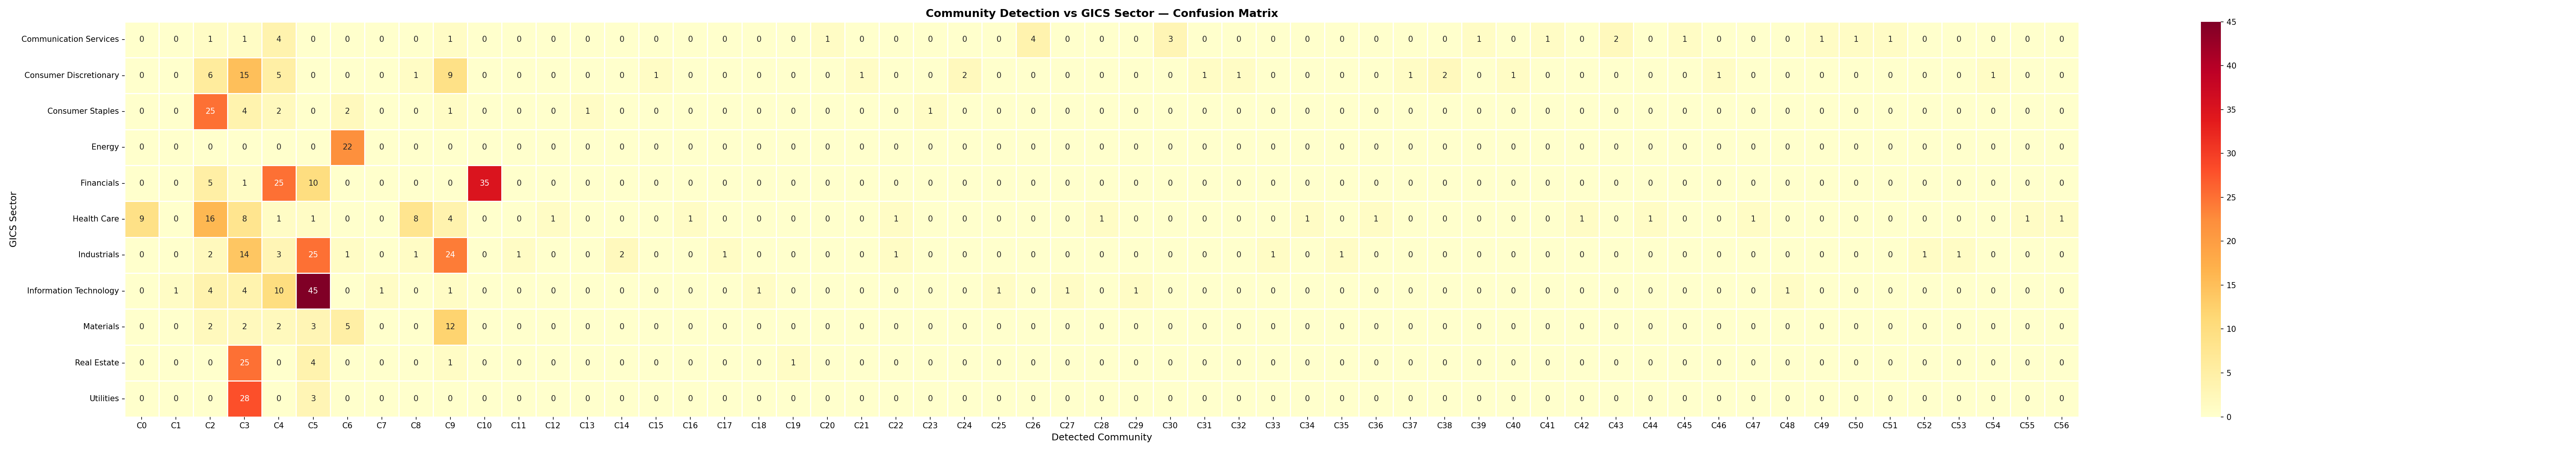
\includegraphics[width=\linewidth,height=0.45\textheight,keepaspectratio]{../../figures/community_vs_sector.png}
            \end{figure}
        \end{column}
    \end{columns}
\end{frame}

% ---------------------------------------------------------
\section{Temporal Dynamics}
% ---------------------------------------------------------
\begin{frame}{Rolling Windows}
    \begin{columns}[c]
        \begin{column}{0.5\textwidth}
            \textbf{Setup}
            \begin{itemize}
                \item 18 overlapping 6-month windows spanning the full 2-year period.
            \end{itemize}
            
            \vspace{0.3cm}
            \textbf{Findings}
            \begin{itemize}
                \item Clustering and modularity increase during stress periods.
                \item The network tightens when macro shocks hit---consistent with ``flight to correlation'' behaviour.
            \end{itemize}
        \end{column}
        
        \begin{column}{0.45\textwidth}
            \begin{figure}
                \centering
                
\includegraphics[width=\linewidth,height=0.7\textheight,keepaspectratio]{../../figures/rolling_window_metrics.png}
                \caption{Structural metrics over rolling windows.}
            \end{figure}
        \end{column}
    \end{columns}
\end{frame}

\begin{frame}{Conclusions}
    \begin{alertblock}{Key Finding}
        The S\&P 500 correlation network is scale-free, small-world, and highly modular---yet systematically vulnerable to targeted attacks on high-betweenness nodes.
    \end{alertblock}
    
    \vspace{0.3cm}
    \textbf{Contributions:}
    \begin{itemize}
        \item \textbf{Filtering}: Market-mode subtraction removes spurious correlations.
        \item \textbf{Null Models}: Configuration model confirms small-worldness beyond degree effects.
        \item \textbf{Validation}: Propagation model tested against three real market events.
    \end{itemize}
\end{frame}

\begin{frame}
    \begin{center}
        \Huge \textbf{Thank You.}
    \end{center}
\end{frame}

\end{document}
